% ════════════════════════════════════════════════════════════════════════════════
%  REPORTE TÉCNICO — PLANTILLA PROFESIONAL
%  Universidad Autónoma de Guadalajara · Ingeniería Mecatrónica
%  
%  Portada de una página + contenido en dos columnas
%  Buenas prácticas LaTeX y estructura profesional
%  
%  Autor: César Manuel Perera Martínez
% ════════════════════════════════════════════════════════════════════════════════

\documentclass[11pt,letterpaper,onecolumn]{article}

% ────────────────────────────────────────────────────────────────────────────────
% CONFIGURACIÓN: Codificación e idioma
% ────────────────────────────────────────────────────────────────────────────────

\usepackage[utf8]{inputenc}
\usepackage[T1]{fontenc}
\usepackage[spanish,es-nodecimaldot]{babel}


% ────────────────────────────────────────────────────────────────────────────────
% TIPOGRAFÍA
% ────────────────────────────────────────────────────────────────────────────────

\usepackage[scaled=0.97]{helvet}
\renewcommand{\familydefault}{\sfdefault}


% ────────────────────────────────────────────────────────────────────────────────
% MATEMÁTICAS Y SÍMBOLOS
% ────────────────────────────────────────────────────────────────────────────────

\usepackage{amsmath}
\usepackage{mathtools}


% ────────────────────────────────────────────────────────────────────────────────
% LAYOUT Y GEOMETRÍA
% ────────────────────────────────────────────────────────────────────────────────

\usepackage{geometry}
\geometry{
  top       = 2.0cm,
  bottom    = 2.0cm,
  left      = 2.0cm,
  right     = 2.0cm,
  headheight = 40pt,
  headsep    = 3ex,
}


% ────────────────────────────────────────────────────────────────────────────────
% FLOTANTES: Figuras, tablas y referencias
% ────────────────────────────────────────────────────────────────────────────────

\usepackage{float}
\usepackage{graphicx}
\graphicspath{{assets/}{figures/}{img/}}

\usepackage{booktabs}
\usepackage{array}
\usepackage{multirow}
\usepackage{caption}
\usepackage{subcaption}
\usepackage{stfloats}


% ────────────────────────────────────────────────────────────────────────────────
% COLORES: Paleta corporativa
% ────────────────────────────────────────────────────────────────────────────────

\usepackage{xcolor}

% Colores corporativos UAG e ingeniería
\definecolor{vinoUAG}   {cmyk}{0.0,0.95,0.70,0.70}  % Rojo oficial UAG
\definecolor{darkText}  {RGB}{30,35,45}            % Texto principal
\definecolor{accentGray}{RGB}{120,120,125}         % Acentos grises
\definecolor{accentDark}{RGB}{25,30,45}            % Gris-azul profundo
\definecolor{bgLight}   {RGB}{250,250,252}         % Fondo claro


% ────────────────────────────────────────────────────────────────────────────────
% UTILIDADES PARA ESPACIOS DE IMÁGENES
% ────────────────────────────────────────────────────────────────────────────────

\newcommand{\placeholderfigure}[2]{%
  \begin{center}
    \fcolorbox{accentGray}{bgLight}{%
      \parbox[c][#1][c]{0.92\linewidth}{%
        \centering\color{accentGray}\small #2
      }%
    }%
  \end{center}
}


% ────────────────────────────────────────────────────────────────────────────────
% TEXTO Y FORMATO
% ────────────────────────────────────────────────────────────────────────────────

\usepackage{ragged2e}
\usepackage{microtype}


% ────────────────────────────────────────────────────────────────────────────────
% LISTAS: Enumeradas e itemizadas
% ────────────────────────────────────────────────────────────────────────────────

\usepackage{enumitem}
\setlist[itemize]{noitemsep, topsep=2pt, leftmargin=*}
\setlist[enumerate]{noitemsep, topsep=2pt, leftmargin=*}


% ────────────────────────────────────────────────────────────────────────────────
% ENCABEZADO Y PIE DE PÁGINA
% ────────────────────────────────────────────────────────────────────────────────

\usepackage{fancyhdr}
\usepackage{etoolbox}

\pagestyle{fancy}
\fancyhf{}
\fancyhead[L]{\small\textcolor{accentGray}{\itshape Ingeniería Mecatrónica}}
\fancyhead[R]{\small\thepage}
\renewcommand{\headrulewidth}{0pt}
\renewcommand{\footrulewidth}{0pt}


% ────────────────────────────────────────────────────────────────────────────────
% SECCIONES: Estilos y espaciado profesional
% ────────────────────────────────────────────────────────────────────────────────

\usepackage[compact]{titlesec}

\titleformat{\section}
  {\normalfont\bfseries\large\color{accentDark}}
  {}
  {0em}
  {\thesection.\hspace{0.5em}}
  [\vspace{-0.8em}{\textcolor{vinoUAG}{\rule{\linewidth}{1.2pt}}}\normalcolor]

\titleformat{\subsection}
  {\normalfont\bfseries\normalsize\color{accentDark}}
  {}
  {0em}
  {\thesubsection.\hspace{0.4em}}

\titleformat{\subsubsection}
  {\normalfont\itshape\small\color{accentGray}}
  {}
  {0em}
  {}

\titlespacing{\section}{0pt}{16pt}{8pt}
\titlespacing{\subsection}{0pt}{10pt}{4pt}
\titlespacing{\subsubsection}{0pt}{6pt}{3pt}


% ────────────────────────────────────────────────────────────────────────────────
% CAJAS DECORATIVAS
% ────────────────────────────────────────────────────────────────────────────────

\usepackage{tcolorbox}
\tcbuselibrary{skins,breakable}


% ────────────────────────────────────────────────────────────────────────────────
% HIPERVÍNCULOS Y REFERENCIAS
% ────────────────────────────────────────────────────────────────────────────────

\usepackage{pdfpages}
\usepackage{subfiles}
\usepackage{appendix}
\usepackage{xurl}
\usepackage[
  colorlinks  = true,
  linkcolor   = vinoUAG,
  urlcolor    = vinoUAG,
  citecolor   = accentGray,
  pdftitle    = {Reporte Técnico},
  pdfauthor   = {Ingeniería Mecatrónica},
]{hyperref}


% ════════════════════════════════════════════════════════════════════════════════
% INICIO DEL DOCUMENTO
% ════════════════════════════════════════════════════════════════════════════════

\begin{document}

\color{darkText}

% ────────────────────────────────────────────────────────────────────────────────
% PORTADA
% ────────────────────────────────────────────────────────────────────────────────

\thispagestyle{empty}

\vspace*{1.0cm}

% Logo de la Universidad Autónoma de Guadalajara (comentado hasta disponibilidad)
% Descomenta las siguientes líneas cuando tengas el archivo del logo
\noindent

\includegraphics[width=0.18\textwidth]{uag1.png}
\hspace{1.0cm}

\noindent
{\huge\bfseries\color{accentDark} Reporte técnico del robot SCARA ROBOEGG}

\vspace{0.5cm}
\noindent
{\large\color{accentGray} Modelado cinemático, calibración, planificación de trayectorias y validación experimental}

\vspace{1.5cm}
\noindent
{\textcolor{vinoUAG}{\rule{\linewidth}{1.5pt}}}

\vspace{1.0cm}

\noindent
\textbf{Autor:}\hspace{0.3cm} César Manuel Perera Martínez y Rebeca Isabel Hernandez Benitez 

\vspace{0.3cm}
\noindent
\textbf{Docente:}\hspace{0.3cm} José Guadalupe Santiago Ovando

\vspace{0.3cm}
\noindent
\textbf{Fecha:}\hspace{0.3cm} \today

\vspace{0.3cm}
\noindent
\textbf{Institución:}\hspace{0.3cm} 
Universidad Autónoma de Guadalajara — Ingeniería Mecatrónica

\vspace{2.0cm}

% Resumen ejecutivo con caja decorativa
\noindent
\begin{tcolorbox}[
  colback  = bgLight,
  colframe = vinoUAG,
  boxrule  = 1pt,
  arc      = 2pt,
  left     = 8pt,
  right    = 8pt,
  top      = 6pt,
  bottom   = 6pt,
  fontupper = \normalsize\color{darkText},
  breakable,
]
\noindent\textbf{\color{vinoUAG}Resumen}

\vspace{0.3cm}

En este proyecto se desarrolló un robot SCARA construido sin kit comercial, con estructura mecánica impresa en 3D, control por Arduino y actuadores paso a paso para los ejes principales, además de un servo para el efector final. El sistema se programó en Python y Arduino para ejecutar trayectorias geométricas, validar una zona segura de trabajo y aplicar calibración persistente del espacio de dibujo.

El reporte documenta la metodología de diseño, los parámetros D-H utilizados para el modelo planar, el código de planificación de trayectorias, la evidencia de construcción, el proceso de calibración y los resultados obtenidos durante las pruebas. También se reservan apartados específicos para evidencias fotográficas del robot terminado, el diseño en SolidWorks y el ensamble físico.

\end{tcolorbox}

\vspace{0.8cm}

\vspace{2.0cm}

% Activar dos columnas para el contenido principal
\twocolumn

\color{darkText}


% ════════════════════════════════════════════════════════════════════════════════
% CONTENIDO PRINCIPAL
% ════════════════════════════════════════════════════════════════════════════════

\section{Introducción}
\justify

El robot SCARA de este proyecto fue desarrollado como una solución mecatrónica de bajo costo y fabricación propia, cumpliendo con la restricción de no utilizar kits comerciales. La meta principal fue construir una plataforma capaz de reproducir trazos geométricos sobre papel mediante control computacional, cinemática inversa y coordinación entre software, electrónica y mecánica.

El sistema integra dos articulaciones rotacionales en el plano $XY$ y un eje discreto para levantar o bajar el instrumento de dibujo. La arquitectura se eligió por su simplicidad cinemática, su repetibilidad y su facilidad de implementación en un entorno académico. A nivel de control, el proyecto se apoya en un programa en Python para el cálculo de trayectorias y en un firmware de Arduino para convertir ángulos en movimiento físico.

Durante el desarrollo se detectó la necesidad de calibrar el modelo geométrico ideal con la realidad mecánica del robot. Por ello, el código incorpora compensación de longitud efectiva, corrección angular y ajustes persistentes del espacio de trabajo, lo que permitió alinear mejor las trayectorias teóricas con el papel real.


% ────────────────────────────────────────────────────────────────────────────────

\section{Objetivos}
\justify

\textbf{Objetivo general.} Construir y validar un robot SCARA funcional, con control por computadora, capaz de trazar figuras geométricas y documentar su evidencia técnica.

\vspace{0.2cm}

\textbf{Objetivos específicos.}
\begin{itemize}
  \item Diseñar y fabricar la estructura mecánica del robot sin recurrir a un kit comercial.
  \item Implementar la cinemática inversa para ubicar el efector final en el plano de trabajo.
  \item Generar trayectorias interpoladas para figuras como triángulo, cuadrado, pentágono y círculo.
  \item Incorporar un sistema de calibración para corregir desplazamientos, escala y rotación del dibujo.
  \item Validar la comunicación serial y el movimiento del robot con firmware en Arduino.
\end{itemize}


% ────────────────────────────────────────────────────────────────────────────────

\section{Metodología}
\justify

El desarrollo se realizó en cinco etapas. Primero se definió la arquitectura mecánica y el alcance del robot a partir de los materiales disponibles: estructura impresa en 3D, motores paso a paso para los dos brazos principales, un servo para el eje Z y una tarjeta Arduino con CNC Shield para el control de potencia.

En la segunda etapa se modeló la cinemática del brazo. El código principal utiliza una longitud efectiva para el segundo eslabón y un ángulo de compensación mecánica para corregir el desfase entre el modelo geométrico ideal y el comportamiento real del mecanismo. También se estableció una zona segura para evitar colisiones con la base o con posiciones fuera del alcance.

La tercera etapa consistió en el desarrollo del firmware de Arduino. El microcontrolador recibe comandos seriales con el formato \texttt{q1,q2,z}, mueve los motores paso a paso con aceleración controlada, posiciona el servo del lápiz y responde con \texttt{OK} al finalizar cada movimiento.

La cuarta etapa fue la calibración. El programa de control guarda un perfil persistente con desplazamiento, escala, rotación y corrección angular. Esto permite ajustar el espacio de dibujo sin modificar el núcleo matemático del robot.

La quinta etapa consistió en pruebas funcionales y documentación. Se ejecutaron trayectorias de distintas figuras, se registraron los ajustes de calibración y se reservó evidencia visual del robot, el diseño CAD y el ensamble.

\subsection{Enfoque de control}

El control se divide en dos bloques: planificación en Python y ejecución en Arduino. Python calcula puntos intermedios, valida seguridad geométrica y envía cada pose al firmware. Arduino traduce los ángulos a pasos físicos y confirma el avance de cada orden con una respuesta serial.

\subsection{Materiales y construcción}

La documentación del proyecto identifica una base mecánica impresa en 3D, motores paso a paso NEMA 17, drivers A4988, CNC Shield, Arduino UNO y un servomotor para el efector final. La electrónica se alimenta con fuente externa de 12 V, mientras que la lógica de control se ejecuta en computadora mediante Python.
 
% ────────────────────────────────────────────────────────────────────────────────

\section{Parámetros D-H}
\justify

Para el movimiento en el plano $XY$, el robot se modeló como un SCARA planar de dos grados de libertad. El eje vertical se maneja como una acción discreta del servo, por lo que en la tabla D-H se documenta el modelo cinemático principal de los dos eslabones y la corrección mecánica usada en el segundo brazo.

\begin{table}[H]
\centering
\caption{Parámetros Denavit-Hartenberg del robot SCARA}
\renewcommand{\arraystretch}{1.2}
\resizebox{\columnwidth}{!}{%
\begin{tabular}{>{\centering\arraybackslash}p{1.2cm}
                >{\centering\arraybackslash}p{2.2cm}
                >{\centering\arraybackslash}p{2.2cm}
                >{\centering\arraybackslash}p{2.0cm}
                >{\centering\arraybackslash}p{3.0cm}}
\toprule
\textbf{Eslabón} & \textbf{$a_i$ [mm]} & \textbf{$\alpha_i$ [deg]} & \textbf{$d_i$ [mm]} & \textbf{$\theta_i$} \\
\midrule
1 & 150.00 & 0 & 0 & $q_1$ \\
2 & 159.94 & 0 & 0 & $q_2 + 20.30^\circ$ \\
\bottomrule
\end{tabular}
}
\end{table}

La corrección angular de $20.30^\circ$ compensa la geometría real del segundo brazo. El modelo usa además una longitud efectiva de $159.94\,\text{mm}$ para representar la distancia cinemática real entre articulaciones.


% ────────────────────────────────────────────────────────────────────────────────

\section{Códigos de planificación de trayectorias}
\justify

La planeación de trayectorias se implementó en Python a partir de una secuencia de vértices por figura. El algoritmo toma cada segmento, interpola puntos intermedios, aplica calibración del espacio de trabajo, verifica seguridad geométrica, calcula cinemática inversa y transmite las poses al Arduino con confirmación serial.

\begin{tcolorbox}[
  colback=bgLight,
  colframe=accentGray,
  boxrule=0.8pt,
  arc=2pt,
  left=6pt,
  right=6pt,
  top=4pt,
  bottom=4pt,
  fontupper=\ttfamily\small,
  breakable,
]
1. Definir la figura mediante vértices en el plano.

2. Interpolar entre puntos con pasos de dibujo y traslado.

3. Aplicar offset, escala y rotación del perfil de calibración.

4. Verificar que el punto esté dentro de la zona segura.

5. Calcular $q_1$ y $q_2$ mediante cinemática inversa.

6. Enviar \texttt{q1,q2,z} por serial y esperar \texttt{OK}.
\end{tcolorbox}

Los bloques principales de implementación se encuentran en las funciones de generación de figuras, interpolación de trayectorias, cálculo de cinemática inversa y sincronización serial. El firmware de Arduino complementa este flujo al convertir ángulos en movimiento físico y devolver la confirmación de cada paso.


% ────────────────────────────────────────────────────────────────────────────────

\section{Resultados}
\justify

Los resultados del sistema pueden resumirse en tres niveles. A nivel de software, el menú de control permite seleccionar figuras y generar trayectorias interpoladas para triángulo, cuadrado, pentágono y círculo. A nivel de firmware, el Arduino acepta cada comando, mueve los actuadores y retorna una confirmación \texttt{OK} para sincronizar el proceso.

A nivel de calibración, el proyecto incorpora un perfil persistente con correcciones de espacio de trabajo y ángulos, lo que permite adaptar el modelo al montaje físico. La existencia de estos parámetros demuestra que el robot no se limitó al modelo teórico, sino que fue ajustado con pruebas reales.

\subsection{Gráficas obtenidas}

En esta sección se colocan las gráficas del comportamiento del robot y de las trayectorias trazadas. Se recomienda incluir, al menos, una gráfica del contorno teórico de las figuras y una comparación con la trayectoria obtenida en la práctica.

\begin{figure}[H]
   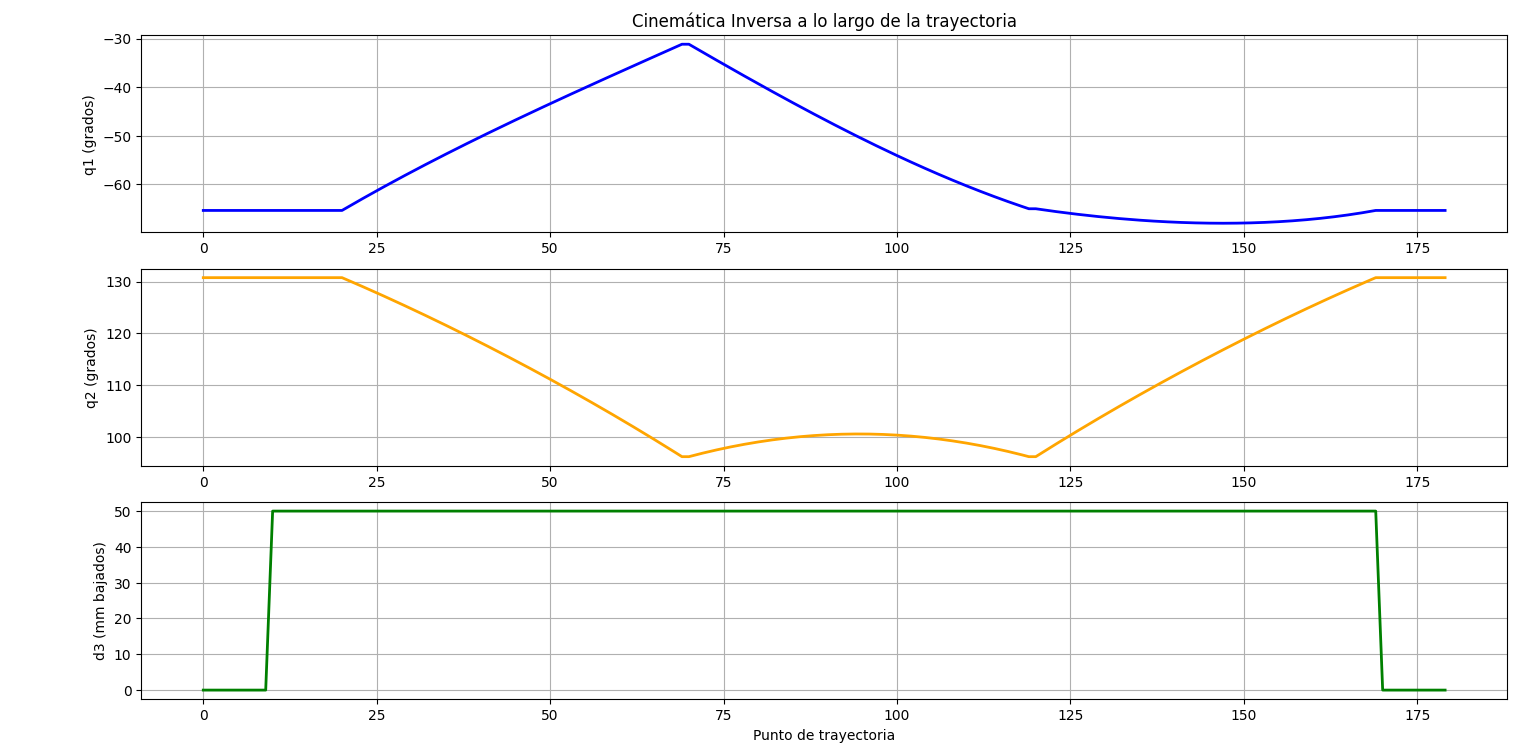
\includegraphics[width=0.95\columnwidth]{figura1.png}
  \caption{Gráfica obtenida durante la planificación de trayectorias.}
\end{figure}

\begin{figure}[H]
  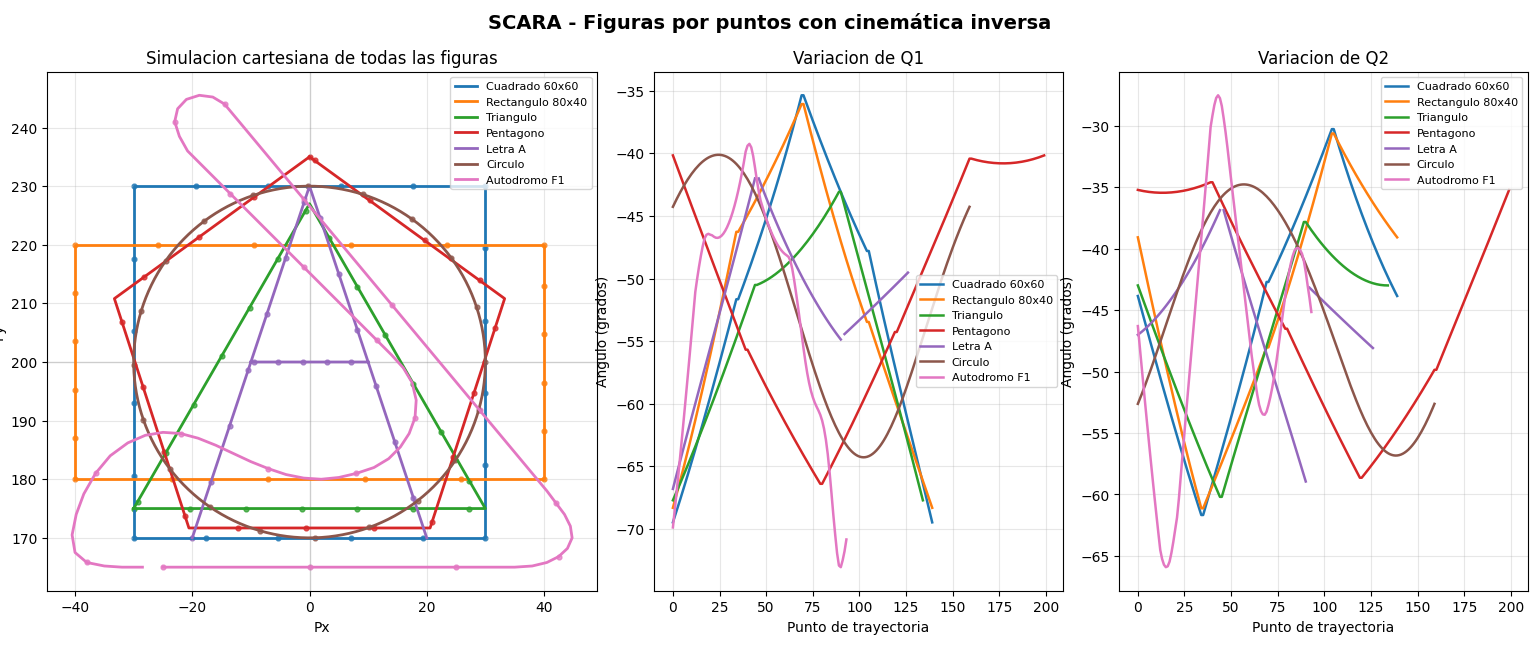
\includegraphics[width=0.95\columnwidth]{figura2.png}
  \caption{Comparación entre resultado esperado y resultado experimental.}
\end{figure}


% ────────────────────────────────────────────────────────────────────────────────

\section{Discusión}
\justify

El desempeño del robot depende de la coincidencia entre el modelo cinemático y la mecánica real. Por esa razón, el uso de un eslabón efectivo y de una compensación angular fue necesario para compensar offsets y holguras del montaje.

La estrategia de planificación por interpolación lineal entre vértices permitió construir figuras cerradas con un comportamiento predecible, aunque el acabado final sigue dependiendo de la precisión del ensamble, de la tensión mecánica de las correas y de la respuesta real del servo al levantar o bajar el lápiz.

El uso de una respuesta serial \texttt{OK} después de cada comando fue clave para evitar desfases entre la computadora y el controlador. Esta decisión simplifica la sincronización y mejora la trazabilidad de las pruebas.


% ────────────────────────────────────────────────────────────────────────────────

\section{Conclusiones}
\justify

El robot SCARA del proyecto cumple con la condición de ser una construcción propia y no un kit comercial. Además, integra mecánica, electrónica y software de forma coherente para resolver el problema de trazado geométrico.

La implementación de cinemática inversa, la validación de seguridad y la calibración persistente hacen que el sistema sea técnicamente defendible y extensible. En particular, el ajuste de longitud efectiva y la compensación angular muestran que hubo iteración real entre diseño y prueba.

Como trabajo futuro, conviene documentar mediciones cuantitativas de error por figura, incluir fotografías de cada prueba y consolidar una bitácora de calibración para fortalecer la evidencia experimental.

\subsection{Robot terminado}

\begin{figure}[H]
  \centering
  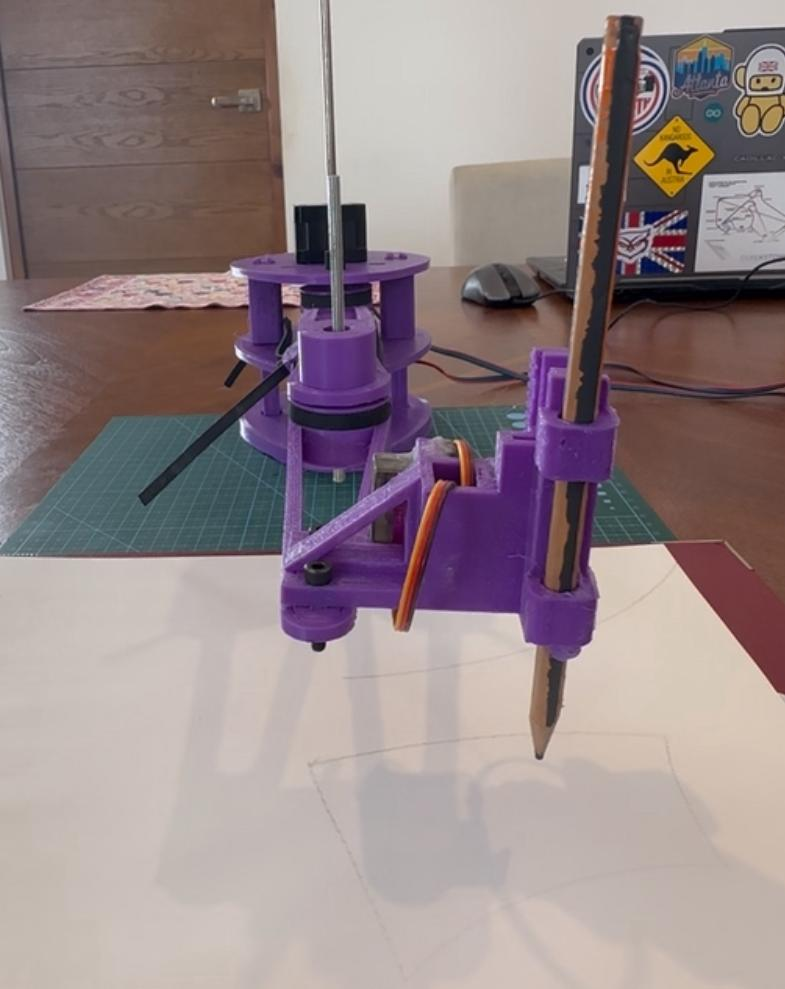
\includegraphics[width=0.95\columnwidth]{figura4.jpeg}
  \caption{Robot ensamblado durante una prueba de trazado.}
\end{figure}
\subsection{Diseño en SolidWorks}

\begin{figure}[H]
  \centering
  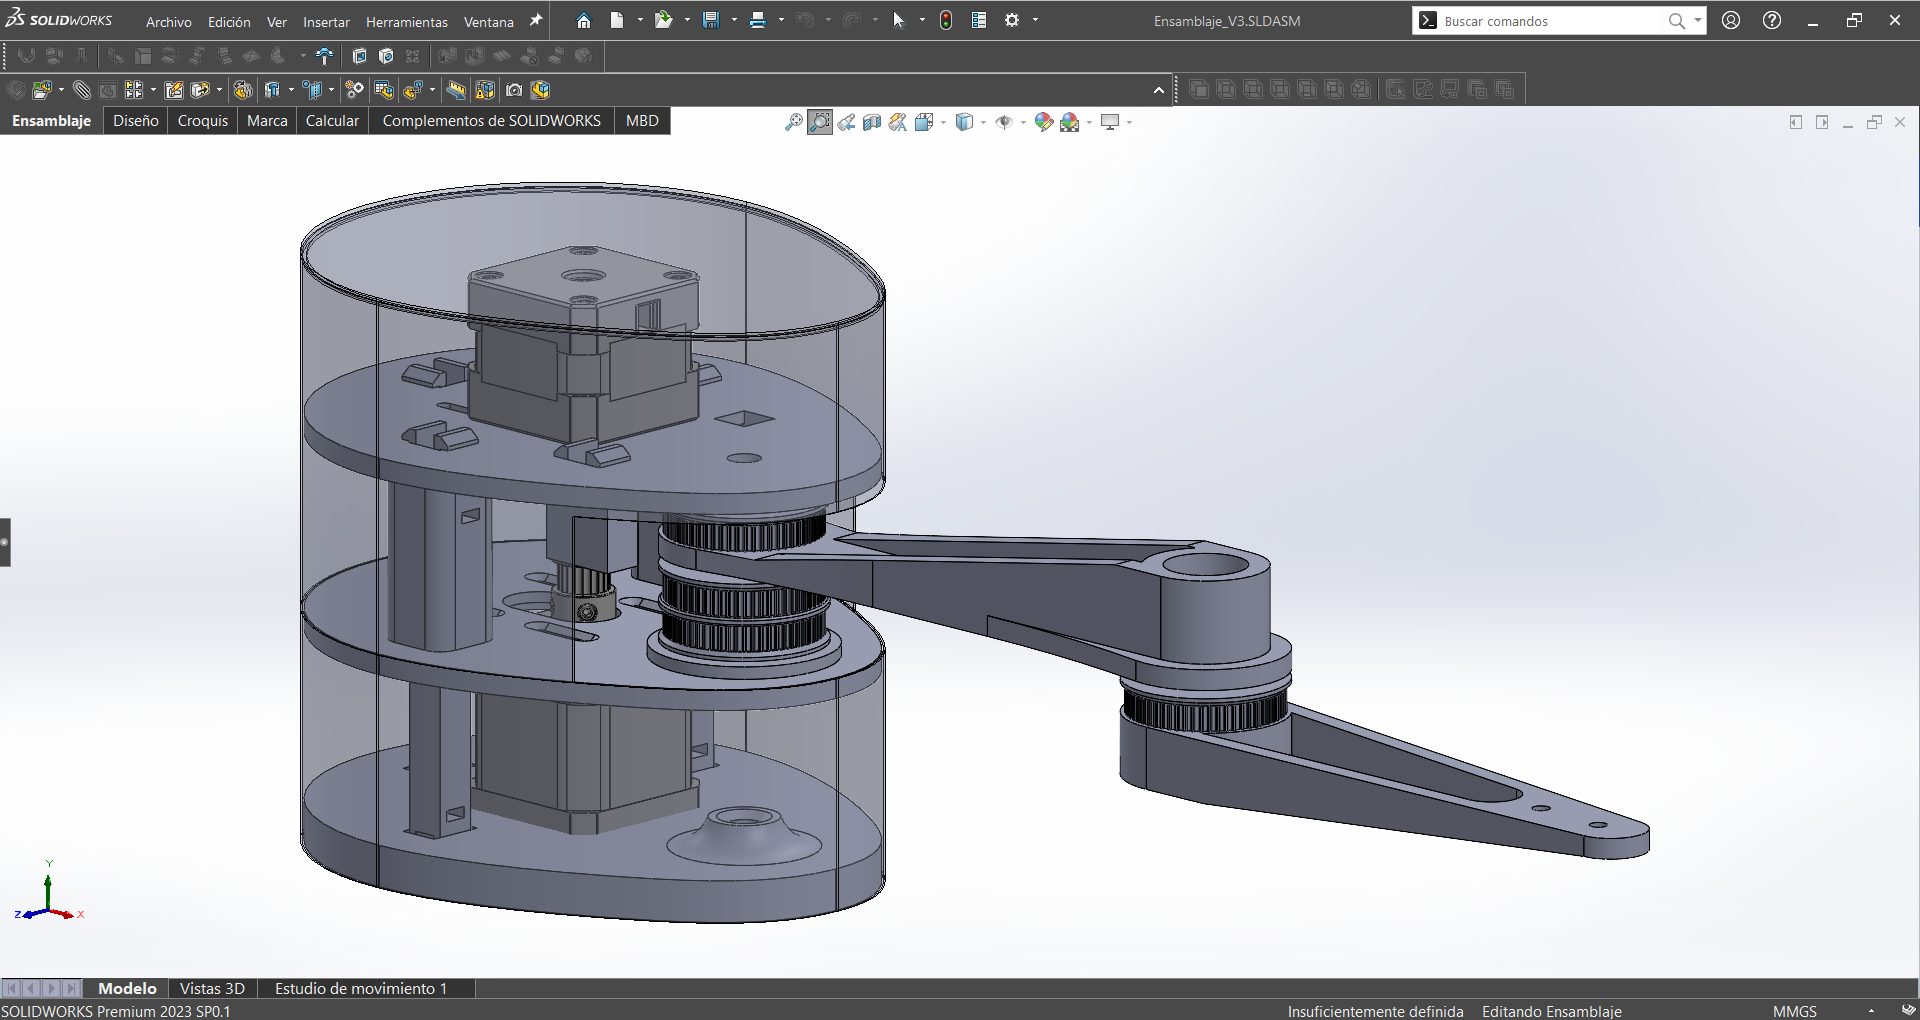
\includegraphics[width=0.95\columnwidth]{figura5.png}
  \caption{Modelo CAD del robot SCARA en SolidWorks.}
\end{figure}

\subsection{Ensamble}

\begin{figure}[H]
  \centering
  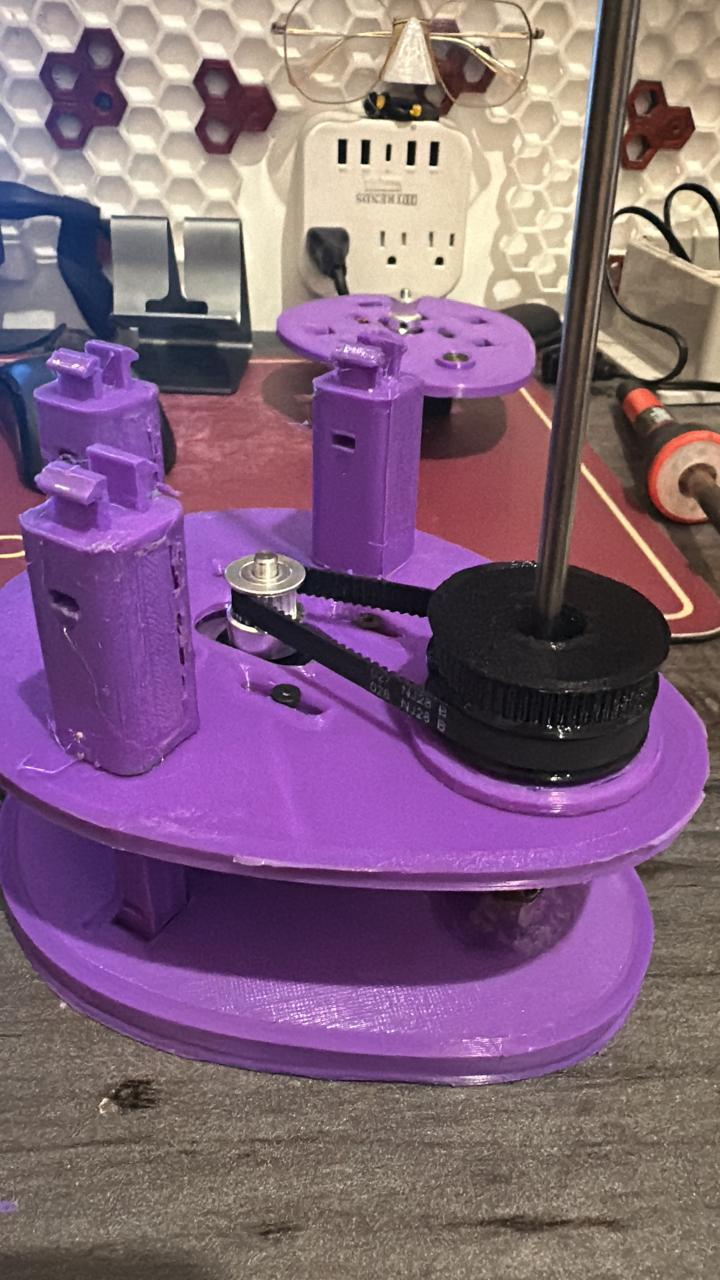
\includegraphics[width=0.95\columnwidth]{figura6.jpeg}
  \caption{Vista general del robot SCARA construido.}
\end{figure}


% ────────────────────────────────────────────────────────────────────────────────

\section{Referencias}
\justify
\small

\begin{enumerate}
  \item Código fuente del control principal del robot SCARA en Python.
  \item Firmware de Arduino para control de motores y servo.
  \item Archivo de calibración persistente del espacio de trabajo.
  \item Instrucciones de electrónica y montaje del proyecto.
\end{enumerate}


% ════════════════════════════════════════════════════════════════════════════════
% FIN DEL DOCUMENTO
% ════════════════════════════════════════════════════════════════════════════════

\end{document}